% -*- latex -*-

%%----------------------------------------------------------------------
\title[systemd]{\emph{\huge systemd}\\[1ex] ``Init on Steroids''}
\author[Andreas Härpfer]{Andreas Härpfer \\
  {\scriptsize \href{mailto:andreas.haerpfer@consol.de}
   {\nolinkurl{(andreas.haerpfer@consol.de)}}}}
\institute{Consol-Akademie}
\date{v2pre, \today}

%% PDF properties
\subject{systemd}
%\keywords{}

\begin{document}

% Load default settings for lstlisting environment.
%% Default style for the lstlisting environment.
\lstset{ %
  language=Clean,				% language
%  basicstyle=\scriptsize\ttfamily,		% fontsize and style
  basicstyle=\ttfamily,
  %xleftmargin=0pt,				% listing indentation
  xleftmargin=1em,				% listing indentation
  %numbers=left,
  numberstyle=\tiny,
  %stepnumber=1,				% lineno stepping
  %numbersep=10pt,                  		% sep of lineno-s
%  backgroundcolor=\color{LightGray},  		% requires \usepackage{color}
  showspaces=false,
  showtabs=false,
  %% Draw a box around the listing and change BG color.
  %frame=single,				% draw frame
%  frame=lrtb,
  %frame=l,
  %framesep=5pt,
  %framerule=1pt,
  tabsize=8,
  captionpos=b,
  breaklines=true,				% auto linebreaking
  breakatwhitespace=true,			% break only at whitespace
}

\lstdefinestyle{numbered}{
  xleftmargin=0.5em,
  numbers=left,
  numberstyle=\tiny,
  %stepnumber=1,
  numbersep=12pt,
  frame=single,
  frame=l,
  framesep=5pt,
  %framerule=1pt,
}



%%----------------------------------------------------------------------
\begin{frame}[plain]
\titlepage
\end{frame}

\begin{frame}{Agenda}
\tableofcontents
\end{frame}

%%----------------------------------------------------------------------
\section[Überblick]{Überblick: Historie, Features, \dots}

\begin{frame}[fragile, allowframebreaks]{Linux-Init bisher}
\begin{block}{Sys\,V-Init}
\begin{itemize}
\item Robuste, einfache Struktur, "`well known"'.
\item Init-Skripte sind Shellskripte (aber viel doppelter Code).
\item Sequentielle Ausführung (langsam).
\item Reihenfolge nur über S- und K-Links in den Runleveln.
\item Keine echten Dependencies.
\item Kein Monitoring/Auto-Restart von Diensten.
\item Nicht Hotplug-aware.
\end{itemize}
\end{block}

\begin{block}{Andere Init-Systeme}
\begin{itemize}
\item Upstart (Ubuntu)
\item BSD-like
\item \dots
\end{itemize}
\end{block}

\framebreak
Interessante Divergenzen: Wie restartet man Apache?

\begin{lstlisting}[style=numbered]
# apachectl restart
# /etc/init.d/apache2 restart
# service apache2 restart
# restart apache2
# service httpd restart
\end{lstlisting}
\end{frame}


\begin{frame}{Was bietet \emph{systemd}\,?}
\begin{block}{Features}
\begin{itemize}
\item Monitoring/Automatische Service-Restarts.
\item Dependencies zwischen Services.
\item Parallelisierter/asynchroner System-Startup (schnell!).
\item Eventbasierte Aktionen (\emph{inetd} und mehr \dots).
\item Deklarative Konfigurationsdateien statt Init-Skripte\\ (einfacher,
übersichtlicher).
\item Funktionalität über Systemgrenzen hinweg (Remote Management,
zentrales Logging) $\rightarrow$ ``Think Cloud"'
\end{itemize}
\end{block}

\begin{block}{Anleihen u.a. bei}
\begin{itemize}
\item \emph{launchd} (Mac OS X)
\item \emph{SMF} (Solaris)
\end{itemize}
\end{block}
\end{frame}


\begin{frame}[fragile]{Adoption als Default-Init-System}
\begin{tabbing}
SUSE Linux Enterprise Server\quad \= Oktober 2014 \kill\\
Fedora \> Mai 2011 \\
openSUSE \> September 2012 \\
Arch Linux \> Oktober 2012 \\
CoreOS \> Oktober 2013 \\
Redhat Enterprise Linux \> Juni 2014 \\
Oracle Linux \> Juli 2014 \\
SUSE Linux Enterprise Server \> Oktober 2014 \\[1ex]
Debian \> geplant für Debian 8 ``Jessie'' \\
Ubuntu \> geplant \\[1ex]
Gentoo \> nicht als Default
\end{tabbing}
\vspace*{1ex}
\hfill{\footnotesize\url{https://en.wikipedia.org/wiki/Systemd#Adoption_and_reception}}
\end{frame}


\begin{frame}{Kontroverse}
\begin{itemize}
\item Bequem, modern, high-level, \dots aber \dots
\item Verletzt KISS-Prinzip.
\item Verwendet spezifische Features des Linux-Kernels\\ $\rightarrow$
nicht auf anderes OS portierbar.
\item Verleibt sich nach und nach andere Tools ein $\rightarrow$
Bloat.\\ (D-Bus, \emph{udev}, \emph{inetd}, \emph{cron}, \dots)
\item Teilweise sehr kontrovers wahrgenommener Entwickler\\ (Lennart
Poettering [jetzt bei Redhat]).
\item \dots
\end{itemize}

\begin{quote}
``It's a bit like if the makers of ovens decided that kitchens would be
easier if the oven was also the fridge, kettle, freezer, dishwasher and
sink.''
\end{quote}
\hfill{\footnotesize\href{http://www.linuxtoday.com/upload/is-systemd-as-bad-as-boycott-systemd-is-trying-to-make-it-140903095011.html}{http://www.linuxtoday.com/upload/is-systemd-as-bad-as\dots}}
\end{frame}

\begin{frame}[plain]
\emph{``People who favour systemd generally use it to get shit done, not
write blog posts about 'freedom of
choice'{}''.}\,\footnote{\url{https://news.ycombinator.com/item?id=7729075}}

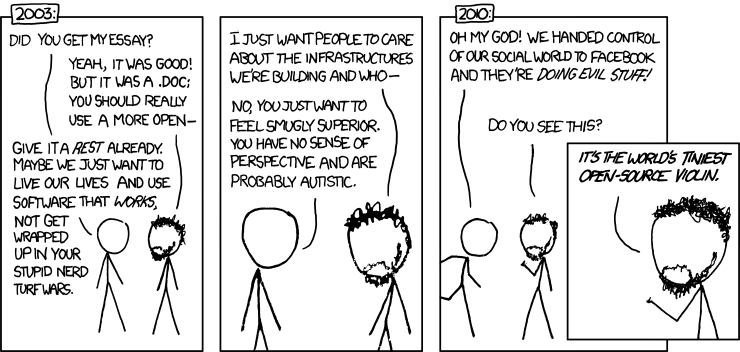
\includegraphics[width=\textwidth]{files/xkcd743-infrastructures.png}
\blfootnote{\url{https://xkcd.com/743/}}
\end{frame}

\begin{frame}{Kontroverse (cont.)}
\begin{quote}
  ``\dots In November 2014, Debian maintainers and Technical Committee
  members Joey Hess, Russ Allbery, Ian Jackson and systemd package
  maintainer Tollef Fog Heen resigned from their positions. All three
  justified their decision on the public Debian mailing list and in
  personal blogs with their exposure to extraordinary stress levels
  related to ongoing disputes on systemd integration within the Debian
  and open source community that rendered regular maintenance virtually
  impossible \dots''

%  \par\vspace{2ex}
%  In December 2014, a fork of Debian, called Devuan, was announced by a
%  group calling themselves the "Veteran Unix Admins". Its intention is
%  to provide a Debian variant without systemd installed by default.''
\end{quote}
\hfill{\footnotesize\url{http://en.wikipedia.org/wiki/Systemd\#History}}
\end{frame}


\begin{frame}[plain]
\vspace*{2ex}
\centerline{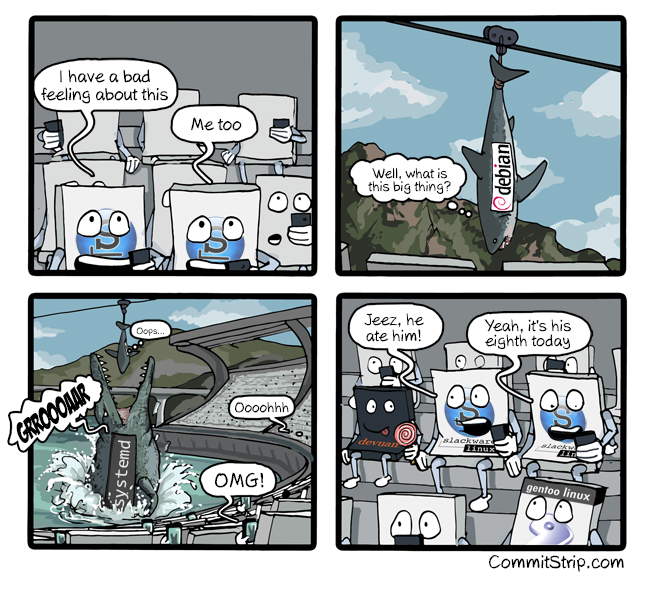
\includegraphics[height=\textheight]
  {files/Strip-SystmeD-650-finalenglish3.png}}
%\hfill{\footnotesize\url{http://www.commitstrip.com/wp-content/uploads/2014/12/Strip-SystmeD-650-finalenglish3.jpg}}
\end{frame}


%%----------------------------------------------------------------------
\section[Basics]{Basics: Dienste verwalten, Targets, \dots}

\begin{frame}{Komponenten/Nomenklatur}
  \begin{columns}[onlytextwidth]
    \begin{column}{0.5\textwidth}
      \begin{block}{systemd}
        \begin{itemize}
          \item systemd (PID=1)
          \item systemctl
          \item Unit-Files
	  \item \emph{/etc/systemd/system.conf}
 	\end{itemize}
      \end{block}

      \begin{block}{Logging}
        \begin{itemize}
          \item systemd-journal
          \item journalctl
	  \item \emph{/etc/systemd/journald.conf}
        \end{itemize}
      \end{block}
    \end{column}

    \begin{column}{0.5\textwidth}
      \begin{block}{Unit-Files}
        \begin{itemize}
	  \item Pkgs: \emph{/lib/systemd/system}
	  \item Lokal: \emph{/etc/systemd/system}
	\end{itemize}
      \end{block}

      \begin{block}{Unit-Typen}
        \begin{itemize}
	  \item target
	  \item service
	  \item socket
	  \item mount/automount/swap
	  \item path
	  \item timer
	\end{itemize}
      \end{block}
    \end{column}
  \end{columns}
\end{frame}

\begin{frame}[fragile, allowframebreaks]{Services --
  \emph{systemctl} Cheatsheet}
\begin{block}{Übersicht}
\begin{lstlisting}
# systemctl
# systemctl list-units --type service
# systemctl list-unit-files --type service
\end{lstlisting}
\end{block}

\begin{block}{Dienste starten, stoppen, etc. (nicht reboot-fest)}
\begin{lstlisting}
# systemctl start   foobar
# systemctl stop    foobar
# systemctl restart foobar
# systemctl reload  foobar
# systemctl status  foobar
\end{lstlisting}
\end{block}

\framebreak
\begin{block}{Dienste reboot-fest aktivieren/deaktivieren:}
\begin{lstlisting}
# systemctl enable      foobar
# systemctl disable     foobar
# systemctl is-enabled  foobar
# systemctl mask|unmask foobar
\end{lstlisting}
\end{block}

\begin{block}{``Deep inspection'' (Unit-Kontext)}
\begin{lstlisting}
# systemctl show foobar
\end{lstlisting}
\end{block}

\framebreak

\begin{block}{Rekonfiguration (nach Installation neuer Unit-Files)}
\begin{itemize}
\item Liest alle Unit-Files neu ein.
\item Baut Dependency-Tree neu auf.
\item Implizit bei \emph{enable} und \emph{disable}.
\end{itemize}
\begin{lstlisting}
# systemctl daemon-reload
\end{lstlisting}
\end{block}

\begin{block}{Boot-up performance}
\begin{lstlisting}
# systemd-analyze [time|blame|plot|...]
\end{lstlisting}
\end{block}
\end{frame}


\begin{frame}[fragile,allowframebreaks]{Targets \xcancel{\normalfont Runlevel}}
\begin{block}{Was sind Targets?}
\begin{itemize}
\item Definierte Laufzeitkonfigurationen ($\approx$~Runlevel).
\item "`Ankerpunkte"' für Dependencies.
\end{itemize}
\begin{lstlisting}
# systemctl list-units --type target
\end{lstlisting}
\end{block}

\begin{block}{Target wechseln}
\begin{lstlisting}
# systemctl isolate some.target
\end{lstlisting}
\end{block}

\begin{block}{Default Target auslesen/setzen}
\begin{lstlisting}
# systemctl get-default
# systemctl set-default some.target
\end{lstlisting}
\end{block}

\framebreak

  \begin{table}
    \small
    \setlength{\aboverulesep}{0pt}
    \setlength{\belowrulesep}{0pt}
    \setlength{\extrarowheight}{0.8ex}
    \begin{tabular}{*{3}{l}}
      \toprule
      \rowcolor{LightBlue}%
      \textbf{Runl.} &
      \textbf{Target Units} &
      \textbf{Description}%
      \bstem\\

      \midrule
      0 & runlevel0.target, poweroff.target &
      Shut down and power off
      \bstem\\

      \midrule
      1 & runlevel1.target, rescue.target &
      Rescue shell (single user)
      \bstem\\

       \midrule
      2 & runlevel2.target, multi-user.target &
      Non-graphical multi-user
      \bstem\\

      \midrule
      3 & runlevel3.target, multi-user.target &
      ditto.
      \bstem\\

      \midrule
      4 & runlevel4.target, multi-user.target &
      ditto.
      \bstem\\

       \midrule
      5 & runlevel5.target, graphical.target &
      Graphical multi-user
      \bstem\\

      \midrule
      6 & runlevel6.target, reboot.target &
      Shut down and reboot
      \bstem\\
      \bottomrule
    \end{tabular}
  \end{table}

\framebreak

\begin{block}{Maintenance Modes}
\textbf{Single-user:} Incl. lokaler Filesysteme und einiger wichtiger
Services.  \emph{Kein Netzwerk!}
\begin{lstlisting}
# systemctl rescue
\end{lstlisting}

\textbf{Emergency-Mode:} Nur \emph{RO} Root-FS \dots falls auch
Rescue-Mode nicht mehr funktioniert:
\begin{lstlisting}
# systemctl emergency
\end{lstlisting}
\end{block}

\framebreak

\begin{block}{Power Management Kommandos}

  \begin{table}
    \small
    \setlength{\aboverulesep}{0pt}
    \setlength{\belowrulesep}{0pt}
    \setlength{\extrarowheight}{0.8ex}
    \begin{tabular}{*{3}{l}}
      \toprule
      \rowcolor{LightBlue}%
      \textbf{Old command} &
      \textbf{New command}%
      \bstem\\

      \midrule
      \texttt{halt} & \texttt{systemctl halt}
      \bstem\\

      \midrule
      \texttt{poweroff} & \texttt{systemctl poweroff}
      \bstem\\

      \midrule
      \texttt{reboot} & \texttt{systemctl reboot}
      \bstem\\

       \midrule
      \texttt{pm-suspend} & \texttt{systemctl suspend}
      \bstem\\

      \midrule
      \texttt{pm-hibernate} & \texttt{systemctl hibernate}
      \bstem\\

      \midrule
      \texttt{pm-suspend-hybrid}\qquad\mbox{} & \texttt{systemctl hybrid-sleep}
      \bstem\\

      \bottomrule
    \end{tabular}
  \end{table}

  Die Kommandos \texttt{runlevel}, \texttt{telinit}, \texttt{shutdown},
  \texttt{reboot}, \dots sind noch vorhanden, sind aber nur Symlinks auf
  \emph{systemctl}.
\end{block}
\end{frame}



%%----------------------------------------------------------------------
\section[Eigene Services]{Demo: Einen eigenen systemd-Service bauen}

\begin{frame}{Abkupfern beim \emph{sshd.service}}
\footnotesize
\lstinputlisting[style=numbered]{files/sshd.service}
\small
(Das korrespondierende Init-Skript ist 160~Zeilen lang [Debian Stable]).
\end{frame}


\begin{frame}{Der erste eigene Service}
\emph{hello.service}
\footnotesize
\lstinputlisting[style=numbered]{files/hello.service}
\end{frame}


\begin{frame}{Hilfreiche Manpages}
  \begin{description}
    \item[systemd.unit(5):] Globale Parameter für die Unit-Konfiguration

    \item[systemd.service(5):] Parameter für Service-Unit

    \item[systemd.exec(5):] Prozess-Environment (inkl.~Settings für
    Logging, TTY, I/O- \& CPU Scheduling, …)

    \item[systemd.kill(5):] Exit-Codes, Restart-Optionen

    \item[systemd.resource-control(5):] Resoure Control Settings für
    die Prozesse des Service (später, advanced feature)

    \item[…] und einige mehr
  \end{description}
\end{frame}


%%----------------------------------------------------------------------
\section[Logging]{Logging in the 21st Century}

\begin{frame}[fragile,allowframebreaks]{\emph{systemd}\,-Logging}
\begin{block}{Features des ``Journal''}
\begin{itemize}
\item Logging auch wenn noch kein \emph{rsyslog} läuft.
\item Strukturierte Logs inkl.~Metadaten, Indizierung, \dots
\item Default Weiterleitung an \emph{rsyslog}, Journal nur im Memory.
\item Separate Persistierung möglich. \\ $\rightarrow$ \texttt{\# mkdir
/var/log/journal}
\item Queries über Systemgrenzen hinweg.
\item \emph{/etc/systemd/journald.conf}
\item journald.conf(5)
\end{itemize}
\end{block}

\framebreak

\begin{block}{Kommandos}
\small
\begin{tabbing}
\quad\=\texttt{\# journalctl -{}-since 12:00 -{}-until 16:00}\quad\= Zeitfenster\kill
\>\texttt{\# journalctl} \> \\
\>\texttt{\# journalctl -r} \> Reverse \\
\>\texttt{\# journalctl -p 4} \> Prio $\ge$ Warning \\
\>\texttt{\# journalctl -u sshd} \> Unit-Filter \\
\>\texttt{\# journalctl -n 1 -o verbose} \> Metadaten \\
\>\texttt{\# journalctl -o json-pretty} \> als JSON \\
\>\texttt{\# journalctl -{}-since 12:00 -{}-until 16:00} \> Zeitfenster 
\end{tabbing}
\end{block}
\end{frame}

% \begin{frame}[fragile]{Unit-Debugging}
% Gesamten Unit-Kontext anzeigen (auch Defaults, die nicht im Unit-File
% stehen):
% \begin{lstlisting}
% # systemctl show foobar
% \end{lstlisting}
% \end{frame}


%%----------------------------------------------------------------------
\section[Advanced]{Advanced Features – Ausblick}

\begin{frame}{Path-Monitoring}
\emph{filemover.path}
\footnotesize
\lstinputlisting[style=numbered]{files/filemover.path}

{\normalsize\emph{filemover.service}}
\lstinputlisting[style=numbered]{files/filemover.service}

\end{frame}


\begin{frame}
\frametitle{User-\emph{systemd}\,\footnote{\emph{launchd} unter OS~X
bietet etwas ähnliches.}}
\begin{itemize}
\item Pro-User Instanz des \emph{systemd} (läuft mit dessen UID).
\item Aktiviert beim Login User-spezifische Services.
\item D-Bus-Kopplung; braucht X11-Session (?).
\end{itemize}
\end{frame}


\begin{frame}{Resource Management}
\begin{itemize}
\item Möglichkeit, Resourcenverbrauch einzelner Dienste etc. zu limitieren.
\item \emph{systemd-cgls}: cgroups Slices,Scopes und Services auflisten.
\item \emph{systemd-cgtop}: Top-artiger Output des Resourcenverbrauchs.
\item systemd.resource-control(5)
\item cgroup Hierarchie unter: \emph{/sys/fs/cgroup/systemd}.
\end{itemize}
\end{frame}


\begin{frame}{Beispiel: I/O eines Service deckeln}
\emph{mybackup.service}
\footnotesize
\lstinputlisting[style=numbered]{files/mybackup.service}
\end{frame}

%%----------------------------------------------------------------------
\begin{frame}[allowframebreaks]{Referenzen}
  \footnotesize
  \begin{itemize}
    \item RHEL 7 System Administrator's Guide
    (Kap.~6)\\ \url{https://access.redhat.com/documentation/en-US/Red_Hat_Enterprise_Linux/7/html/System_Administrators_Guide/}

    \item \emph{systemd}\,-Manpages online:\\
%    \url{http://www.freedesktop.org/software/systemd/man/}
    \url{http://0pointer.de/public/systemd-man/}

    \item \emph{Das Init-System Systemd}, Lennart Poettering, Kay
    Sievers, Thorsten Leemhuis.  Zweiteiliger Überblicksartikel auf
    \emph{heise.de} mit einigen weiterführenden Links.\\
    \url{http://www.heise.de/open/artikel/Das-Init-System-Systemd-Teil-1-1563259.html}\\
    \url{http://www.heise.de/open/artikel/Das-Init-System-Systemd-Teil-2-1563461.html}

    \item Systemd-Projektseite auf \emph{freedesktop.org}; viele
    weiterführende Links:\\
    \url{http://www.freedesktop.org/wiki/Software/systemd/}

    \framebreak
    
    \item \emph{systemd for Administrators}, Serie von Artikeln im Blog
    von Lennart Poettering (mittlerweile 21 Teil!); viele
    Architektur-Details:\\
    \url{http://0pointer.net/blog/archives.html}

    \item \emph{systemd in Debian}, Tollef Fog Heen, Michael Biebl,
    FOSDEM 2013\\
    \url{https://people.debian.org/~biebl/fosdem/debian-systemd.pdf}
    
  \end{itemize}
\end{frame}


\begin{frame}[plain]
  \centerline{\Huge Fragen?}
\end{frame}

\end{document}

